\chapter{Интеграл Римана.}
Последняя тема в этом семестре. Продолжаем развитие и углубление школьных идей. Правда, подход к интегралу несколько иной, чем в школе.
\section{Интегральные суммы.}
$\bullet$ \textit{\textbf{Разбиением отрезка} $[a; b]$ назовём конечную систему точек $ a = x_0, x_1, x_2, \ldots, x_{n - 1}, x_n = b $ этого отрезка такую, что $ a_0 \neq x_0 < x_1 < \ldots < x_{n - 1} < x_n = b $.} 
$$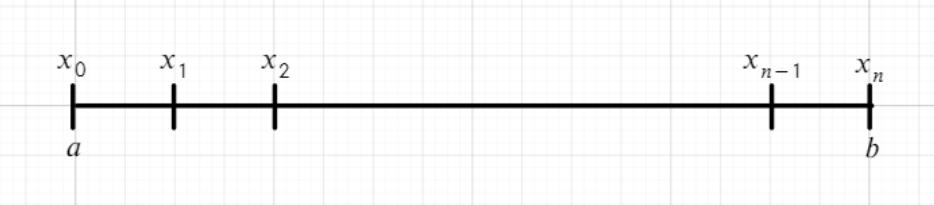
\includegraphics[scale=0.5]{images/img40.png}$$
Обозначать разбиение будем символом $ \{x_k\}_{k = p}^{k = n} $,  или $ \{x_k\}_{0}^{n} $, или $ \{x_k\} $.\\\\
$\bullet$ \textit{Отрезки $ [x_{k - 1}; x_k] $ --- \textbf{отрезки разбиения}.}\\\\ Длину отрезка $[x_{k - 1}; x_k] $ обозначим $ \Delta x_k $, т.е. $ \Delta x_k ::= x_k - x_{k - 1} $. Отметим, что $ \Delta x_k > 0,$ для любого k $\Delta x_k ::= x_k - x_{k - 1} $.\\\\\
$\bullet$ \textit{Обозначим $ \delta ::= \underset{k}{\max} \{ \Delta x_k \}$ и будем называть $\delta$ \textbf{диаметром разложения}. Диаметр разложения --- это наибольшая из длин всех отрезков.}\\\\
Можно построить бесконечно много разбиений с одним и тем же диаметом $ \delta $. \\\\
Рассмотрим теперь $ f : [a; b] \to {\Rm} $. \\\\
Выберм на каждом из отрезков разбиения $ [x_{k - 1}; x_k] $ произвольным образом точку $ \xi_k $, т.е. $ \xi_k \in [x_{k - 1}; x_k]$, $k = 1,2,\ldots, n $  и построим интегральную сумму.
$$\upvarsigma ::= \sum\limits_{k = 1}^n f(\xi_1) \Delta x_1 + f(\xi_2) \Delta x_2 + \ldots + f(\xi_n) \Delta x_n.$$
Ясно, что величина, значение, этой интегральной суммы зависит как от способа разбиения отрезка $[a; b]$, так и от выбора точке  $ \xi_k$. \\\\
\section{Интеграл Римана.}
$\bullet$ \textit{Число $J$ называется \textbf{пределом интегральных сумм} $ \upvarsigma $  при диаметре разбиения $ \delta \to 0 $, если $ \forall \eps > 0$, $\exists \delta_{\eps}$, $\forall \{x_k\}$, $\delta \leqslant \delta (\eps)$ и $\forall \xi_k \in [x_{k - 1}; x_k] $ выполняется неравенство $ |\sigma - J |\leqslant \eps.$}\\\\
Другими словами, $\forall \eps > 0 $  должно найтись $ \delta (\eps) $ такое, что все интегральные суммы, соответствующие произвольным разбиениям отрезка $[a; b]$  с диаметром меньшим, чем $\delta (\eps) $, при произвольном выборе точек $\xi_k $, должны попасть на орезок $ [J - \eps; J + \eps]$. \\\\
Записываем $ J = \lim\limits_{\delta \rightarrow{} 0}\upvarsigma $. \\\\
Для введённого таким образом предела имеет место М-лемма. 
\begin{mlemma}
	Если $$ \forall \eps > 0, \exists \delta_{\eps} > 0, \forall \{x_k\}, \forall \xi_k \in [x_{k - 1}; x_k], 0 < \delta \leqslant \delta (\eps) \Rightarrow |\upvarsigma - J| \leqslant M\eps ,$$ где $M$ не зависит ни от $ \eps $, ни от $ \delta $, ни от $ \{ x_k \} $, ни от $ \xi_k$, то $ \upvarsigma \rightarrow{} J $, при $ \delta \rightarrow{} 0 $.  
\end{mlemma}
\begin{Proof}
	Доказательство аналогично оказательству всех М-лемм.
\end{Proof}\\\\
Отличие этого рассматриеваемого предела от рассмотренных ранее состоит в том, что одному и тому же $ \delta $ соответсвует бесконечно много  $ \upvarsigma $. Тем не менее и введённый таким образом предел обладает всеми свойчтвами, характерными для обычного предела.
Например, имеет место
\begin{theorem}[Аналог критерия Гейне]
	Для того, чтобы $ \upvarsigma \rightarrow{} J $ при $ \delta \rightarrow{} 0 $ необходимо и достаточно, чтобы для $ \forall $  последовательности разбиений $ \{ x_{k_m} \} $, при $ \forall $ выборе точке $ \xi_{k_m}, \upvarsigma_m \rightarrow{} J $  при $ \delta \rightarrow{} 0 $.
\end{theorem}
\begin{Proof}
	Доказательство произвоится аналогично доказательству критерия Гейне для предела функции.
\end{Proof}\\\\
Сформулированная теорема позволяет распространить на $ \lim\limits_{\delta \rightarrow{} 0} \upvarsigma $ обычные свойства предела последовательности. \\\\
$\bullet$ \textit{Если $ \lim\limits_{\delta \rightarrow{} 0} \upvarsigma $ существует, то функцию f  называют \textbf{интегрируемой в смысле Римана} на отрезке $[a; b]$. Число $ J = \lim\limits_{\delta \rightarrow{} 0} \upvarsigma $ называют \textbf{интегралом Римана} или \textbf{определённым интегралом} и обозначают $ \int\limits_a^b f(x)dx $.} \\\\
Таким образом $$ \int\limits_a^b f(x)dx = \lim\limits_{\delta \rightarrow{} 0} \upvarsigma = \lim\limits_{\delta \rightarrow{} 0} \sum\limits_{k = 1}^{\infty} f(\xi_k) \Delta x_k .$$
$\bullet$ \textit{Множество всех интегрируемых в смысле Римана функций на отрезке $[a; b]$ будем обозначать $\mathcal{R}([a; b])$.}\\\\
Слова $"$функция интегрируема в смысле Римана на отрезке $[a,b]"$ символически запишутся так $f\in\mathcal{R}([a; b])$.\\\\
$a$ --- нижний предел интегрирования, $b$ --- верхний предел интегрирования, $f$ --- подынтегральная функция, $f(x)dx$ --- подынтегральное выражение, $x$ --- переменная интегрирования.\\\\
Поскольку мы пока не будем рассматривать другого интеграла, кроме интеграла Римана, условимся для краткости говорить просто $"$интеграл$"$ и $"$интегрируемая функция$"$ вместо слов $"$интеграл Римана$"$ и $"$функция интегрируемая в смысле Римана$"$.\\
\begin{example}
	$f(x) = c$ $\fa x \in [a;b]$.\\
	$\upvarsigma= \sum\limits^n_{k=1}c\Delta x_k = c(b-a)\Ra c \inRim$ и $\int\limits_a^b cdx = c(b-a)$, в частности, $\int\limits^b_ab-a, \int\limits^b_a0dx = 0$.
\end{example}
\section{Необходимое улосвие интегрируемости.}
Допустим, что $f$ задана на $[a;b]$, но неограничена на этом отрезке. Возьмем произвольное разбиение $\{x_k\}$ отрезка $[a;b]$. Тогда найдется отрезок разбиения $[x_{l-1};x_l]$, на котором функция неограничена.\\\\
Фиксируем все $\xi_k$, крое $\xi_l$. За счет выбора $\xi_l$ всегда можно добиться того, что интегральная сумма $\upvarsigma$ будет сколь угодно большой по модулю. Так как это справедливо для любого разбиения, то $f$ не может быть интегрируемой на $[a;b]$. Вывод:
\begin{theorem}
	[Необходимое улосвие интегрируемости]
	Для $f\inRim$ необходимо и достаточно, чтобы $f$ была ограничена на $[a;b]$. Коротко: $f\inRim \Rightarrow f$ ограничена на $[a;b]$.
\end{theorem}
Однако, как показывает следующий пример, ограниченности недостаточно для  интегрируемости.\\
\begin{example}
	$f(x) = D(x) = \begin{cases}0, x\text{ --- иррациональное},\\
		1, x\text{ --- рациональное}
	\end{cases}$.\\\\
	\textbf{Функция Дирихле.}\\\\
	Рассмотрим ее на отрезке $[0;1]$. Для любого разбиения отрезка $[0;1]$ $\{x_k\}$ за счет выбора точек $\xi_k$ можно добиться того, чтобы $\upvarsigma = 0$ ($\xi_k$ --- иррациональное) и $\upvarsigma = 1$ ($\xi_k$ --- рациональное). Пoэтому у $\upvarsigma$ не может быть предела $\Ra$ $D(x) \not\in\mathcal{R}([0;1])$, хотя $D(x)$ и ограничена.
\end{example}\\\\
В дальнейшем рассматриваем только ограниченные функции (если не оговорено противное).
\section{Критерий Коши интегрируемости по Риману.}
Наряду с интегральной суммой $\upvarsigma$, составленной для разбиения $\{x_k\}$ с диаметром $\delta$ и точками $\xi_k$, рассмотрим другую интегральную сумму $\tau = \sum\limits^m_{r=1}f(\eta_r)\Delta t_r$, составленную для разбиения $\{t_r\}^m_0$ отрезка $[a;b]$ с диаметром разбиения $\mu$, где $\eta_r \in [t_{r-1};t_r]$.
\begin{theorem}
	[Критерий Коши]
	Для того, чтобы функция $f\inRim$ необходимо и достаточно, чтобы $\fa \eps > 0$, $\exists \delta_\eps > 0$ такое, что при любых разбиениях $\{x_k\}$ и $\{t_r\}$ и $\fa \xi_k \in [x_{k-1}; x_k]$ и $\fa \eta_r\in [t_{r-1};t_r]$ из $\delta \leq \delta_\eps$ и $\mu \leq \delta_\eps\Ra |\upvarsigma - \tau| \leq \eps.$
\end{theorem}\begin{Proof}
	
\end{Proof}
\section{Необходимое условие Дарбу интегрируемости.}
Помимо уже доказанного необходимого условия есть и другие. К рассмотрению одного из них сейчас и переходим.\\\\
Пусть $f:[a;b]\to \Rm$. Как известно, колебание функции $f$ на $[a;b]$ есть величина $$\omega(f; [a;b]) = \underset{[a;b]}{\sup}f - \underset{[a;b]}{\inf}f.$$
Колебание функции можно также представить и в виде 
$$\omega(f; [a;b]) = \underset{\xi,\eta\in[a;b]}{\sup}|f(\xi) - f(\eta)| = \underset{\xi,\eta\in[a;b]}{\sup}(f(\xi) - f(\eta)).$$
Построим теперь разбиение $\{x_k\}$ отрзка $[a;b]$ и обозначим $\omega_k ::= \omega (f; [x_{k-1};x_k]) $.\\\\
$\bullet$ Интегральным колебанием $f$ по данному разбиению называют число $$\Omega ::= \sum\limits^n_{k=1}\omega_k\Delta x_k.$$
Каждому разбиению отвечает одно единственное интегральное колебание.
$$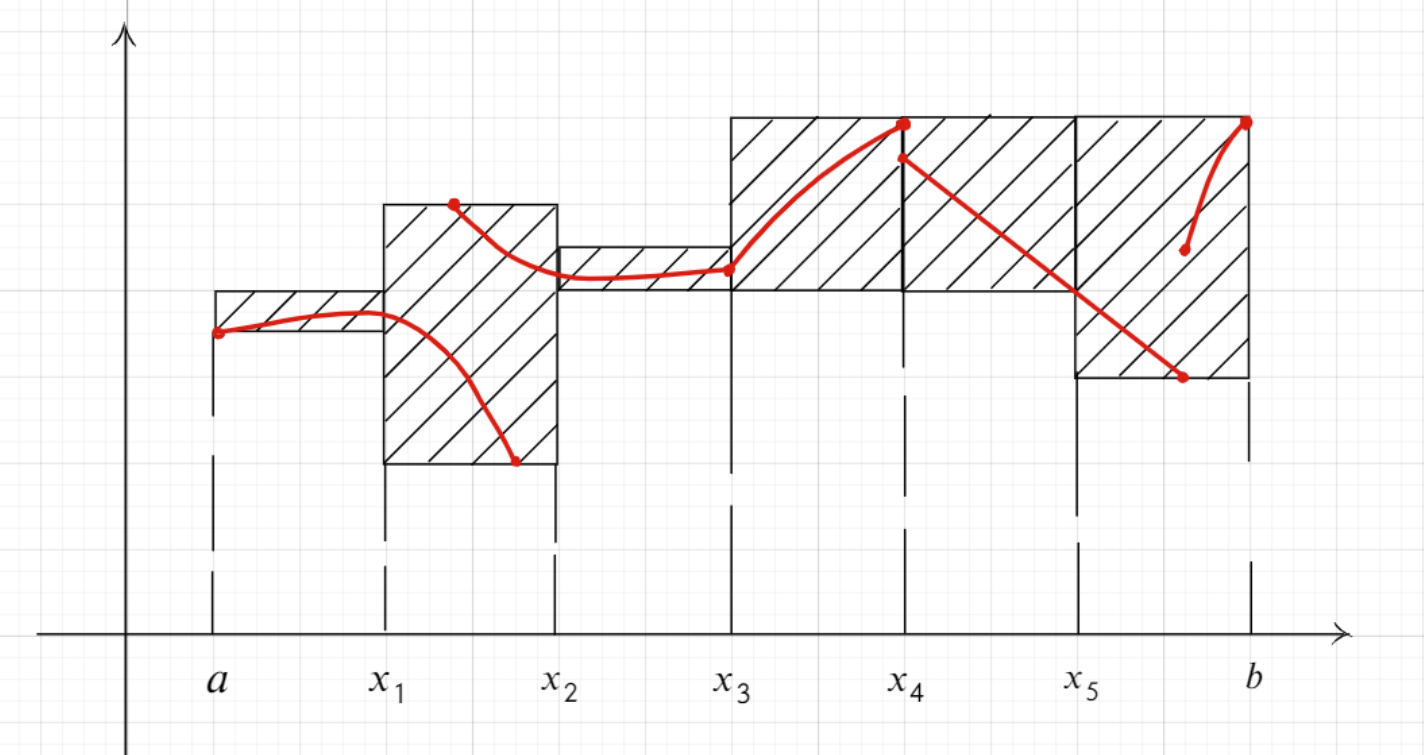
\includegraphics[scale=0.5]{images/img41.png}$$
Если $f$ неограничена, то при каждом разбиении найдётся отрезок, на котором колебание $f$ бесконечно и, поэтому, для каждого разбиения и интегральное колебание бесконечно. Далее рассматриваем только ограниченные функции.\\\\
Предположим теперь, что $f\inRim$, и составим две интегральные суммы $\sigma$ и $\tau$ функции $f$ по одному и тому же разбиению $\{x_k\}$. Тогда $$\sigma - \tau = \sum_{k=1}^{n}f(\xi_k)\Delta x_k - \sum_{k=1}^{n}f(\eta_k)\Delta x_k = \sum_{k=1}^{n}(f(\xi_k) - f(\eta_k))\Delta x_k$$ 
Согласно критерию Коши интегрируемости 
$$\forall \varepsilon > 0,\ \exists \delta_\varepsilon > 0,\ \forall \delta \le \delta_\varepsilon \Rightarrow |\sigma - \tau| \le \varepsilon,\ \forall \xi_k;\ \forall \eta_k$$
Таким образом, $|\sum\limits_{k=1}^{n}(f(\xi_k) - f(\eta_k))\Delta x_k| \le \varepsilon$  для $\forall \delta \le \delta_k$, при любом выборе точек $\xi_k$ и $\eta_k$. Отсюда следует, что
$$\sup_{\xi_k, \eta_k} |\sum_{k=1}^{n}(f(\xi_k) - f(\eta_k))\Delta x_k| \le \varepsilon$$
Но точки $\xi_k$ и $\eta_k$ выбираются независимо друг от друга, поэтому предыдущее неравенство равносильно такому 
$$\sup_{\xi_k, \eta_k} |\sum_{k=1}^{n}(f(\xi_k) - f(\eta_k))\Delta x_k| = \sup_{\xi_k, \eta_k} \sum_{k=1}^{n}|(f(\xi_k) - f(\eta_k))|\Delta x_k =$$ $$ = \sum_{k=1}^{n}\sup_{\xi_k, \eta_k}|(f(\xi_k) - f(\eta_k))|\Delta x_k = \sum_{k=1}^{n}\omega_k \Delta x_k = \Omega \le \varepsilon.$$
\begin{theorem}[Необходимое условие Дарбу интегриуремости]
	Если $f\inRim \Rightarrow \forall \varepsilon > 0, \exists \delta_\varepsilon > 0, \forall \delta \le \delta_\varepsilon \Rightarrow \Omega \le \varepsilon$. Или, другими словами, если $f$ интегрируема на отрезке $[a;b]$, то все интегральные колебания $f$ для разбиений с достаточно маленькими диаметрами сколь угодно малы.
\end{theorem}
\section{Представление и оценка разности двух интегральных сумм.}
Наряду с интегральной суммой $\sigma = \sum\limits_{k=1}^{n}f(\xi_k)\Delta x_k$, составленной для разбиения $\{x_k\}$ с диаметром $\delta$ и точками $\xi_k$, рассмотрим интегральную сумму $\tau = \sum\limits_{r=1}^{m}f(\eta_r)\Delta t_r$, составленную для разбиения ${\{t_r\}}^m_0$ отрезка $[a;b]$ с диаметром $\mu$ и точками $\eta_r \in [t_{r - 1}; t_r]$.\\\\
Через $\Delta_{kr}$ обозначим длину промежутка $[x_{k - 1}; x_k] \cap [t_{r - 1}; t_r]$. Если это пересечение пусто, то $\Delta_{kr} = 0$.\\\\
Очевидно: $\sum\limits_{k=1}^{n}\Delta_{kr} = \Delta t_r$,  $\sum\limits_{r=1}^{m}\Delta_{kr} = \Delta x_k$,  $\sum\limits_{k=1}^{n} \sum\limits_{r=1}^{m} \Delta_{kr} = b - a$.\\\\
Интегральные суммы $\sigma$ и $\tau$ можно представить так:
$$\sigma = \sum_{k=1}^{n}f(\xi_k)\Delta x_k = \sum_{k=1}^{n}f(\xi_k) \sum_{r=1}^{m} \Delta_{kr} = \sum_{k=1}^{n} \sum_{r=1}^{m} f(\xi_k) \Delta_{kr}  $$
$$\tau = \sum_{r=1}^{m}f(\eta_k)\Delta t_r = \sum_{r=1}^{m}f(\eta_k) \sum_{k=1}^{n} \Delta t_r = \sum_{k=1}^{n} \sum_{r=1}^{m} f(\eta_k) \Delta_{kr}  $$
Тогда разность $\sigma - \tau$  запишется в виде
$$\sigma - \tau = \sum_{k=1}^{n} \sum_{r=1}^{m}(f(\xi_k) - f(\eta_k))\Delta_{kr} $$
Здесь суммирование ведётся по всем $k$ и $r$, даже по тем, для которых $\Delta_{kr} = 0$
\begin{lemma}[$\Delta$-лемма]
	$$\sigma - \tau = \underset{|\xi_k - \eta_r| \le \delta + \mu}{\sum_{k, r}}(f(\xi_k) - f(\eta_r))\Delta_{kr}.$$
\end{lemma}
\begin{Proof}
	Предположим, что $[x_{k-1}; x_k]\cap[t_{r-1}; t_r]\neq \varnothing$, то есть $\exists \gamma$ являющейся общей для двух отрезков. Тогда\begin{center}
		$|\xi_k - \gamma| \le \delta$, так как $\xi_k,\gamma \in [x_{k-1}; x_k]$;\\
		$|\eta_k - \gamma| \le \mu$, так как $\eta_k,\gamma \in [t_{k-1}; t_k]$.
	\end{center}
	Значит $$|\xi_k - \eta_k| \le |\xi_k - \gamma| + |\eta_k - \gamma| \le \delta + \mu.$$
	Если же $|\xi_k - \eta_k| \ge \delta + \mu$, то указанные промежутки не имеют общих точек и значение $\Delta_{k_r} = 0$. Таким образом, из исходной суммы выброшена часть тех слагаемых, для которых $\Delta_{k_r} = 0$. 
	$$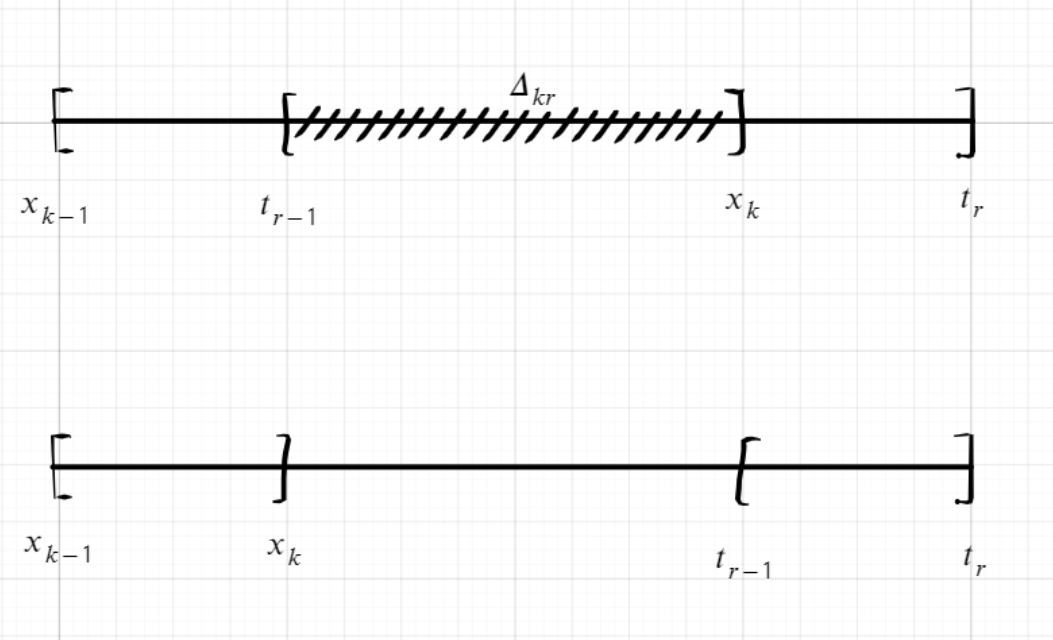
\includegraphics[scale=0.5]{images/img42.png}$$
\end{Proof}
\begin{lemma}[$\Omega$-лемма]
	Пусть $|f(x)| \le A$; $\forall x \in [a;b]$. Пусть $\omega_r^*$ -- колебание функции $f$ на отрезке $[t_{k-1}; t_k]$ и $P$ --- интегральное колебание $f$ по $\{t_r\}$, то есть $P = \sum\limits_{r=1}^{m}\omega_r^* \Delta t_r$. Тогда 
	$$|\sigma - \tau| \le P + 2A(m - 1)\delta.$$
\end{lemma}
\begin{Proof}
	На основании $\Delta$-леммы
	$$|\sigma - \tau| = \underset{|\xi_k - \eta_r| \le \delta + \mu}{|\sum_{k, r}}(f(\xi_k) - f(\eta_r))\Delta_{kr}| \le \underset{|\xi_k - \eta_r| \le \delta + \mu}{\sum_{k, r}}|f(\xi_k) - f(\eta_r)|\Delta_{kr}$$
	Разобьем эту сумму на две ${\sum}_1$ и ${\sum}_2$. К ${\sum}_1$ отнесём слагаемые, отвечающие таким $\Delta_{kr}$, для которых $[x_{k-1}; x_k]\subset[t_{r-1}; t_r]$, а к ${\sum}_2$ -- все остальные слагаемые.\\\\
	\underline{Оценим ${\sum}_1$:}\\\\
	Поскольку $[x_{k-1}; x_k]\subset[t_{r-1}; t_r]$, то $\xi_k, \mu_r \in [t_{r-1}; t_r]$, а тогда $|f(\xi_k) - f(\eta_r)| \le \omega_r^*$ и $${\sum}_1 \le \underset{|\xi_k - \eta_r| \le \delta + \mu}{\sum} \omega_r^* \Delta t_r \le \sum_{r=1}^{m}\omega_r^* \sum_{k=1}^{n}\Delta_{kr} = \sum_{r=1}^{m}\omega_r^* \Delta t_r  = P.$$
	\underline{Оценим ${\sum}_2$:}\\\\
	В ${\sum}_2$ попадут лишь такие слагаемые, для которых каждый отрезок $[x_{k-1}; x_k]$ содержит внутри себя по крайней мере одну точку вида $t_r$. Таких промежутков будет не больше, чем $m - 1$, так как имеется только лишь $m - 1$ внутренних точек $t_r$. Длина каждого из отрезков $\Delta_{kr} \le \delta$. Поэтому ${\sum}_2 \le \sum(|f(\xi_k)| - |f(\eta_r)|)\Delta_{kr} \le 2A(m - 1)\delta$.\\\\
	Объединяя оценки для ${\sum}_1$ и ${\sum}_2$, получаем утверждение леммы.
\end{Proof}
\section{Критерий Дарбу интегрируемости}
\begin{theorem}[Достаточное условие Дарбу интегрируемости]
	Если для $\forall \epsilon > 0$ $\exists$ разбиение, по которому интегральное колебание $f$ не превосходит $\epsilon$, то $f \inRim$.
\end{theorem}
\begin{Proof}
	Зададим $\forall \epsilon > 0$. Согласно условию существует разбиение $\{t_r\}_0^m$ отрезка $[a;b]$ с интегральным колебанием $P \le \epsilon$ . Зафиксируем это разбиение. Возьмём любое другое разбиение $\{t_{x_k}\}$ с диаметром $\delta \le \epsilon$. Тогда $|\sigma - \tau| \le \epsilon + 2A(m - 1)\epsilon$ (по $\Omega$-лемме).\\\\
	Теперь возьмём ещё одно разбиение $\{z_{x_j}\}$ с диаметром $\lambda \le \epsilon$ и составим интегральную сумму $\bar \sigma$. Тогда на основании той же $\Omega$-леммы $|\bar \sigma - \tau| \le \epsilon + 2A(m - 1)\epsilon$ .\\\\
	Поэтому $|\sigma -\bar \sigma| \le |\bar \sigma - \tau| + |\sigma - \tau| \le 2\epsilon + 4A(m - 1)\epsilon = M \cdot \epsilon$, где $M = 4A(m - 1)$. А тогда на основании критерия Коши $ \Rightarrow f \inRim.$
\end{Proof}
\begin{theorem}[Критерий Дарбу интегрируемости по Риману]
	Для $f \inRim$ необходимо, чтобы интегральное колебание функции $f$ по любому достаточно мелкому  разбиению было сколь угодно малым и достаточно, чтобы интегральное колебание могло быть сделанным по некоторому разбиению сколь угодно малым ( то есть $\forall \epsilon > 0, \exists \{x_k\} \Rightarrow \Omega \le \epsilon$).
\end{theorem}
Заметим, что если $\Omega = \varepsilon$ хотя бы пo одному разбиению, то тогда оно будет сколь угодно малым по всем разбиениям с достаточно малым диаметром.
\section{Классы интегрируемых функций}
Все функции в этом пункте предполагаем ограниченными.
\begin{enumerate}
	\item 
	$f \in \mathcal{C}([a;b]) \Rightarrow f \inRim$.
	\begin{Proof}
		Всякая функция, непрерывная на отрезке, вместе с тем ограничена на нем. Кроме того, на основании теоремы Кантора $f$ и равномерно непрерывна на $[a;b]$. Тогда $$\forall \varepsilon > 0, \exists \delta(\varepsilon) > 0, \forall x', x'' \in [a;b], |x'-x''| \leqslant \delta(\varepsilon) \Rightarrow |f(x') - f(x'')|\leqslant \varepsilon$$
		Построим разбиение $\{x_k\}$ отрезка $[a;b]$ с диаметром $\delta$ меньшим, чем $\delta(\varepsilon)$.\\\\ Тогда $\sup\limits_{[x_{k - 1};x_k]} |f(x')-f(x'')| \leqslant \varepsilon$ и, следовательно, $\omega_k \leqslant \varepsilon$. Оценим интегральное колебание $f$ по этому разбиению $\{x_k\}$.
		$$\displaystyle\Omega = \sum\limits_{k = 1}^{n} \omega_k \Delta x_k \leqslant  \sum\limits_{k = 1}^{n} \varepsilon\Delta x_k = \varepsilon(b - a).$$
		По критерию Дарбу интегрируемости $f \inRim$
	\end{Proof}
	\item \textit{Если $f$ монотонна на $[a;b]$ и ограничена $\Rightarrow f \inRim$.}
	\begin{Proof}
		Пусть, например, $f$ возрастает на $[a;b]$. Тогда $\omega_k = f(x_k) - f(x_{k - 1}) \geqslant 0$  на любом разбиении $\{x_k\}$.\\\\
		Рассмотрим 
		\begin{multline*}
			\displaystyle\Omega = \sum\limits_{k=1}^{n}(f(x_k)- f(x_{k - 1}))\Delta x_k \leqslant \sum\limits_{k=1}^{n}(f(x_k)- f(x_{k - 1}))\delta = \\  = \delta(f(x_1) - f(x_0) + f(x_2) - f(x_1) + ... + f(x_n) - f(x_{n - 1})) = \delta (f(x_n) - f(x_0)) = (f(b) - f(a))\delta
		\end{multline*}
		За счет выбора $\Omega$ можно сделать сколь угодно малым, поэтому по критерию Дарбу $f \inRim$. Для убывающей функции аналогично.
	\end{Proof}
	\item \textit{Если $f$ кусочно-монотонна и ограничена на $[a;b]$, то $f \inRim$. Подробнее: если $[a;b]$ можно разбить на конечное число промежутков, на каждом из которых $f$ монотоннa, то $f \inRim$.}
	\begin{Proof}
		На каждом из промежутков (пусть их $p$) функция интегрируема в смысле Римана. Поэтому можно построить разбиение каждого промежутка так, что интегральное колебание $f$ на каждом из промежутков не превосходит $\varepsilon$. Построим разбиение $[a;b]$, объединив разбиения всех промежутков. Тогда интегральное колебание $f$ по этому разбиению $\Omega \leqslant p \cdot \varepsilon$. По критерию Дарбу $f \inRim$.
	\end{Proof}
	\item
	\textit{Если $f$ ограничена на $[a;b]$ и $\forall [\alpha; \beta] \subset ]a;b[ \ f \in\mathcal{R}([\alpha;\beta])$, то  $f \inRim$}
	\begin{Proof}
		Для $\varepsilon > 0 \Rightarrow f \in \mathcal{R}([a+\varepsilon; b - \varepsilon])$.
		\\\\
		Возьмем разбиение отрезка $[a + \varepsilon; b - \varepsilon]$ так, чтобы $\Omega_{[a+\varepsilon; b - \varepsilon]} \leqslant \varepsilon$. Тогда $\Omega_{[a;b]} \leqslant 2A\varepsilon + \varepsilon + 2A\varepsilon$ и используем критерий Дарбу.
	\end{Proof}
$$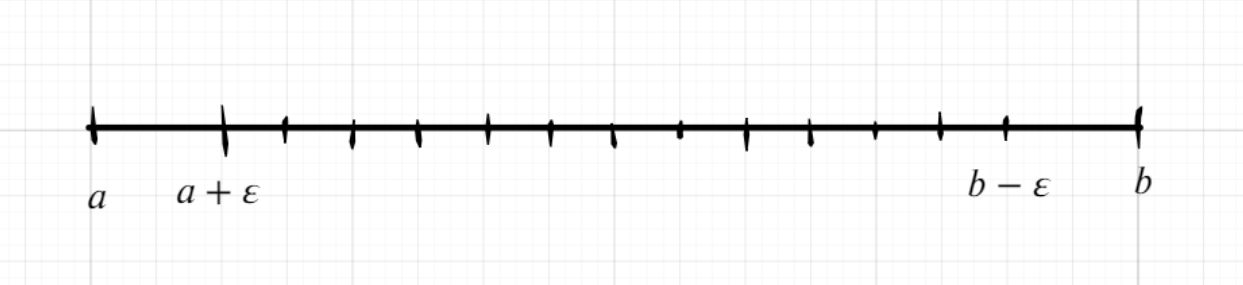
\includegraphics[scale=0.5]{images/img43.png}$$
	$$\omega_0 = f(\xi_1) - f(\eta_1) \Rightarrow |\omega_0| \leqslant 2A$$
	$$\omega_n = 2A$$
	\item
	\textit{Если $f$ ограничена $[a;b]$ на и имеет лишь конечное число точек разрыва, то $f \inRim$}
	\\\
	\begin{Proof}
		В частности, если $f$ ограничена на $[a;b]$ и непрерывна на $]a;b[$, то в силу 4 $f \inRim$.\\
		В общем случае $[a;b]$ можно разбить на конечное число отрезков, на каждом из которых $f \in  \mathcal{R}$, а затем доказательство продолжнается и заканчивается, как в 3.
	\end{Proof}
	\begin{corollary}
		Отсюда сразу же следует, что если $f = 0$ на $[a;b]$, за исключением конечного числа точек, то $f \inRim$ и тогда $\int\limits_a^b f(x)dx = 0$.
	\end{corollary}
	\begin{corollary}
		Если $f \inRim$ и если изменить значение $f$ в конечном числе точек, то $f \inRim$ и величина интеграла не изменится.
	\end{corollary}
\end{enumerate}
\section{Критерий Лебега интегрируемости в смысле Римана.}
$\bullet$ \textit{Говорят, что множество $E\subset\Rm$ \textbf{имеет меру нуль(является множеством меры нуль)} в смысле Лебега, если для $\forall \varepsilon > 0$ его можно покрыть конечной или счетной системой интервалов, суммарная длина которых не превосходит $\varepsilon$.}\\\
Т.е. если $l_i, i = 1, 2, ...$ длины интервалов покрытия, то $l_1 + l_2 + ... = \sum \limits_{i = 1}^{\infty} l_i < \varepsilon$.
\begin{example}
	\begin{enumerate}
		\item одноточечное множество
		\item конечное число точек
		\item счетное множество точек $x_1, x_2, ..., x_n,...$
		$$\frac{\varepsilon}{2} + \frac{\varepsilon}{2^2}+ ... +\frac{\varepsilon}{2^n} = \frac{\frac{\varepsilon}{2}}{1 - \frac{1}{2}} = \varepsilon$$
		\item Множество $\Q$ --- множество меры нуль.
	\end{enumerate}
\end{example}
\\\
$\bullet$
\textit{Если некоторое свойство выполнено в любой точке множества $X$, кроме, быть может, точек множества меры нуль, то говорят, что это свойство \textbf{имеет место почти всюду на множестве $X$}  или \textbf{почти во всех точках множества $X$}.}
\begin{theorem}[Критерий Лебега]
	Ограниченная на отрезке функция интегрируема на нем тогда и только тогда, когда $f$ непрерывна почти во всех точках отрезка $[a;b]$ (т.е. когда множество ее точек разрыва есть множество меры нуль)
\end{theorem}
\begin{corollary}
	Если множество точек разрыва ограниченной на отрезке $[a;b]$ функции конечно или счетно, то $f \inRim$.
\end{corollary}
\chapter{Основные свойства интегрируемых функций.}
\section{Линейность интеграла.}
\begin{theorem}
	Если $f, g \inRim$, то и $\alpha f + \beta g \inRim$, где $\alpha, \beta$ --- постоянные, $\alpha, \beta \in \Rm$, причем $$\int \limits_{a}^{b}(\alpha f(x) + \beta g(x))dx = \alpha\int \limits_a^b f(x)dx + \beta\int \limits_a^b g(x)dx.\eqno{(1)}$$
\end{theorem}
\begin{Proof}
	Составим интегральную сумму для интеграла в левой части (1) и преобразуем ее.
	\begin{multline*}
		\sigma_{\alpha f + \beta g} = \sum \limits_{k = 1}^{n} (\alpha f + \beta g) (\xi_k)\Delta x_k
		= \alpha \sum \limits_{k = 1}^{n} f(\xi_k)\Delta x_k + \beta \sum \limits_{k = 1}^{n} g (\xi_k) \Delta x_k = \alpha \sigma_f + \beta\sigma_g\end{multline*}
	Устремим диаметр рабиения к нулю. Предел правой части существует и равен линейной комбинации интегралов, значит существует и предел левой части и он должен быть равен пределу правой части. Это и значит, что $\alpha f + \beta g \inRim $ и выполняется (1).
\end{Proof}
\section{Аддинитивность интеграла}
Пусть $f \inRim$. Возьмем любой $[\alpha ; \beta] \subset [a; b]$.\\\\
Для $\forall \varepsilon > 0$ можно указать такое разбиение $\{x_k\}$ отрезка $[a;b]$, что $\Omega_{[a;b]} \leqslant \varepsilon$. Разбиение $\{x_k\}$ отрезка $[a;b]$ порождает разбиение отрезка  $[\alpha ; \beta]$ и тогдa $\Omega_{[\alpha;\beta]} \leqslant \Omega_{[a;b]} \leqslant \varepsilon$, поскольку $\Omega_{[\alpha;\beta]}$ --- чaсть $\Omega_{[a;b]}$.\\\\
Следовательно, в силу достаточной части критерия Дарбу $f \in  \mathcal{R}([\alpha;\beta])$. В частности, если $f \inRim$, то для $\forall c \in [a;b] \Rightarrow f \in  \mathcal{R}([a;c]) \wedge f \in  \mathcal{R}([c;b])$.\\\\
Верно и обратное. Пусть $\forall c \in [a;b] \Rightarrow f \in  \mathcal{R}([a;c]) \wedge f \in  \mathcal{R}([c;b])$. Тогда $f \inRim$.
\\\\
\begin{Proof}
	Возьмем разбиения промежутков $[a;c]$ и $[c;b]$ такие, чтобы интегральные колебания на каждом из промежутков не превосходили $\epsilon$; то есть $\Omega[a;c] \leq \epsilon$ и $\Omega[c;b] \leq \epsilon$. Рассмотрим теперь разбиение отрезка $[a;b]$, являющееся объединением разбиений отрезков $[a;c] \wedge [c;b]$. Тогда $\Omega[a;b] = \Omega [a;c] + \Omega[c;b] \leq 2\epsilon$
\end{Proof}\\\\
Если функция интегрируема, то для вычисления интеграла можно взять любую последовательность разбиений, лишь бы $\delta \rightarrow 0$ и $\forall \xi_{k}$.
В частности разбиения можно выбирать так, чтобы $c$, где $a< c < b$, все время была одной из точек разбиения.
В этом случае $$\sigma_{[a;b]}=\sigma_{[a;c]}+\sigma_{[c;b]}.$$
Переходя в этом равенстве к пределу при $\delta \rightarrow 0$, получим
$$\int\limits_a^b f(x)dx = \int\limits_a^c f(x)dx + \int\limits_c^b f(x)dx \eqno (2)$$
Это равенство и выражает аддитивность интеграла.\\\\
Мы, определяя интеграл Римана, считали, что $a<b$, когда рассматривали $f:[a;b] \rightarrow \Rm$. Однако от этого ограничения можно отказаться при составлении итнегральных сумм, только считать, что $\Delta x_k > 0$, если $a < b$ и $\Delta x_k < 0$, если $a > b$. Тогда интегральные суммы будут отличаться только знаком. По этим соображениям принимаются следующие соглашения:
\begin{center}
	если $a > b$, то $\int\limits_a^b f(x)dx ::= -\int\limits^b_a f(x)dx$\\
	и так же $\int\limits_a^a f(x)dx = 0$
\end{center}
С учетом этих соглашений нетрудно видеть, что (2) имеет место не только при $a < c <b$, но и при любом взаимном расположении точек $a$, $b$ и $c$, причем слудет потребовать существование двух интегралов, тогда существует и третий и справедливо равенство. Это равенство можно записать и в таком виде:
$$\int\limits_a^b f(x)dx + \int\limits_a^c f(x)dx + \int\limits_c^b f(x)dx = 0.$$
\section{Оценка модуля интеграла.}
\begin{theorem}
	Если $a \leq b$ и $f \inRim$, то $\left|f\right| \inRim$ и справедливо неравенство $$\left| \int\limits_a^b f(x)dx \right|  \leq \int\limits_a^b \left| f(x) \right| dx$$
	Если при этом $\left| f(x) \right| \leq A$, то $$\left| \int\limits_a^b f(x)dx \right| \leq A(b-a).$$
\end{theorem}
\begin{Proof}
	При $a=b$ утверждение очевидно, поэтому считаем $a<b$. Интегрируемость $\left| f \right|$ следует из очевидного неравенства $\omega_{\left| f \right|} \leq \omega_f$, что влечет за собой $\Omega_{\left| f \right|} \leq \Omega_f \leq \epsilon$ и работает критерий Дарбу. Для интегральных же сумм будет справедлива следующая оценка:
	$$\left| \sum_{k=1}^n f(\xi_k)\Delta x_k \right| \leq \sum_{k=1}^n \left| f(\xi_k) \right| \Delta x_k \leq \sum_{k=1}^n A\cdot \Delta x_k$$
	Переходя в этом равенстве к пределу, получаем требуемое.
\end{Proof}
\section{Монотонность интеграла.}
\begin{theorem}
	Если $a \leq b$; $f, g \inRim$ и $f(x) \leq g(x)$ $\forall x \in [a;b]$, то $$\int\limits_a^bf(x)dx \leq \int\limits_a^b g(x)dx$$
\end{theorem}
\begin{Proof}
	Случай $a=b$ очевиден.\\\\
	Пусть $a<b$, тогда $\sum\limits_{k=1}^n f(\xi_k)\Delta x_k \leq \sum\limits_{k=1}^n g(\xi_k)\Delta x_k$. Переходим к пределу при $\delta \rightarrow 0$.
\end{Proof}
\begin{corollary}
Если $a \leq b, f \inRim$ и $f(x) \geq 0$ на $[a;b]$, то $\int\limits_a^b f(x) \geq 0$ на $[a;b]$, то $\int\limits_a^b f(x)dx \geq 0$.
\end{corollary}
\begin{Proof}
	Вытекает из теоремы при $g=0$.
\end{Proof}
\begin{corollary}
Если $A \leq f(x) \leq B$ и $f(x) \in R([a;b])$, то $A(b-a) \leq \int_a^b f(x)dx \leq B(b-a)$
\end{corollary}
\begin{Proof}
	Очевидно.
\end{Proof}
\begin{corollary}
Если $f \in R([a;b])$, $m = \underset{[a;b]}{\inf f}$, $M = \underset{[a;b]}{\sup f}$, то $\exists \mu \in [m;M]$, что $$\int_a^bf(x)dx = \mu(b-a)$$
\end{corollary}
\begin{Proof}
	$a=b$ очевидно.\\\\
	$a < b$ по следствию 2.\\\\
	$$m(b-a) \leq \int\limits_a^bf(x)dx \leq M(b-a) \Rightarrow m \leq \frac{1}{b-a}\cdot \int\limits_a^bf(x)dx \leq M.$$
	Положим $\mu = \frac{1}{b-a}\cdot \int\limits_a^bf(x)dx$.
\end{Proof}\\\\
$\bullet$\textit{ Число $\mu$ назовем \textbf{средним значением} функции на $[a;b]$.}
\section{Теоремы о среднем.}
\begin{theorem}[Первая теорема о среднем днем]
	Если $f \in \mathcal{C}([a;b])$, то $\exists \xi \in [a;b]$ такая, что $$\int_a^bf(x)dx = f(\xi)(b-a).$$
\end{theorem}
\begin{Proof}
	По следствию 3 $\exists \mu$, что $\int\limits_a^bf(x)dx = \mu(b-a)$, где $m \leq \mu \leq M$. По теореме о промежуточном значении для непрерывной функции $\exists \xi \in [a;b]$, что $f(\xi) = \mu$.
\end{Proof}
\begin{theorem}[Вторая теорема о среднем]
	Пусть $f, g \in \mathcal{C}([a;b]), g(x) \geq 0$ (или $g(x) \leq 0$, то $\exists \xi \in[a;b]$, что $\int\limits_a^bf(x)g(x)dx = f(\xi)\int\limits_a^b g(x)dx$
\end{theorem}
\begin{Proof}
	$a=b$ равенство очевидно (любое $\xi$).\\\\
	Пусть $a<b$ и для определенности $g(x) \geq 0$.
	Так как $m \leq f(x) \leq M$, где $m = \inf f$, $M = \sup f$, то $mg(x) \leq f(x)g(x) \leq M g(x)$ и на основании монотонности интеграла $$m \int\limits_a^b g(x)dx \leq \int\limits_a^bf(x)g(x)dx \leq M\int_a^b g(x)dx.$$
	Если $\int\limits_a^b g(x)dx = 0$, то очевидно, что утверждение теоремы очевидно.\\\\
	Пусть $\int\limits_a^b g(x)dx \neq 0$ ($\int_a^b g(x)dx > 0$. Тогда $$m \leq \frac{\int\limits_a^b f(x)g(x)dx}{\int\limits_a^b g(x)dx} \leq M$$
	По теореме о промежуточном значении $\exists \xi \in [a;b]$, что $f(\xi) = \frac{\int\limits_a^b f(x)g(x)dx}{\int\limits_a^b g(x)dx}$, что и доказывает теорему.
\end{Proof}\\\\
\textbf{Замечание}.
Иногда доказанную теорему называют первой теоремой о среднем, а второй теоремой о среднем называют такую теорему:
\begin{theorem}
	Если $f, g \inRim$ и $g$ - монотонная на $[a;b]$ функция, то $\exists \xi \in [a;b]$ такая, что $$\int\limits_a^b(f\cdot g)(x)dx = g(a)\cdot \int\limits_a^{\xi}f(x)dx + g(b)\cdot \int\limits_{\xi}^bf(x)dx$$
	Эту формулу называют также \textbf{формулой Бонне} (1819-1892) --- француз.
\end{theorem}
\section{Еще несколько свойств интеграла.}
\begin{enumerate}
	\item \textit{Интеграл от нечетной функции по симметричному промежутку равен нулю.}
	\begin{Proof}
		Составим интегральную сумму, производя разбиение $[-a;a]$ симметричное и выбирая точки $\xi_k$ симметрично началу координат. Тогда в силу равенства $f(-x) = -f(x)$ вытекает, что $\sigma = 0 \Ra I = 0$.
		\end{Proof}
	\item \textit{Интеграл от четной функции по симметричному промежутку равен удвоенному интегралу по половине промежутка.}
	\begin{Proof}
		$\sigma_{[-a;a]} = 2\sigma_{[0;a]}$ в силу $f(-x) = -f(x)$.
		\end{Proof}
	\item \textit{Если $f\in \mathcal{C}([a;b])$, $f(x) \geq 0$, причем $f\not\equiv 0$ на $[a;b]$, то $\int\limits_a^bf(x)dx > 0$.}
	\begin{Proof}
		Так как $f\not\equiv 0\Ra \exists x_0 : f(x_0) > 0$. По теореме о стабилизации знака $\exists \delta >0 : f(x) > 0$ $\forall x \in [x_0-\delta; x_0 + \delta]$. Тогда $$\int\limits_a^bf(x)dx = \int\limits_a^{x_0-\delta}f(x)dx +\int\limits_{x_0+\delta}^{x_0-\delta}f(x)dx+ \int\limits_{x_0+\delta}^bf(x)dx > 0,$$
		так как $\int\limits_{x_0+\delta}^{x_0-\delta}f(x)dx = f(\xi)$, $2\delta > 0$ по теореме о среднем.
		\end{Proof}
	\begin{corollary}[Признаки тождественного обращения в нуль непрерывной функции]
		\begin{enumerate}
			\item Если $f(x)\geq 0$, $f(x) \in \mathcal{C}([a;b])$ и $\int\limits_a^bf(x)dx = 0$, то $f \equiv 0$.
			\item Если $f(x) \in \mathcal{C}([a;b])$, $\int\limits_a^bf^2(x)dx = 0$, то $f \equiv 0$.
		\end{enumerate}
		\end{corollary}
	\item \textit{Если $f\inRim$, то при изменении значений функции в конечном числе точек $g$ будет $g\inRim$ и $\int\limits_a^bf(x)dx = \int\limits_a^g(x)dx$.}
	\begin{Proof}
		Интегрируемость $g$ следует из класса $IV$. Разобъем $[a;b]$ измененными точками на конечное число частей. На каждой из них $f$ интегрируема по $IV$. По свойству аддитивности $g$ интегрируема на $[a;b]$. Равенство интегралов вытекает из возможности выбора нужным образом точек $\xi_k$.
		\end{Proof}
	\item \textit{Если $f,g \inRim$, то $f\cdot g \inRim$.}
	\begin{Proof}
		Так как $f,g \inRim \Ra |f(x)|\leq A$, $|g(x)|\leq B$. Оценим разность \begin{multline*}
			|f(x')g(x') - f(x'')g(x'')| = |f(x')g(x') - f(x')g(x'') + f(x')g(x'') - f(x'')g(x'')| \leq\\\leq |f(x')|\cdot |g(x')-g(x'')| + |g(x'')|\cdot |f(x') - f(x'')|.
			\end{multline*}
		Отсюда следует, что колебание функции $f\cdot g$ удовлетворяет неравенсту $$\omega_{fg}\leq A\omega_g + B\omega_f.$$
		Зададим $\epsilon > 0$ и построим разбиение отрезка $[a;b]$, интегральные колебания по которому функций $f$ и $g$ не превосходят $\eps$. Это возможно, так как функции $f,g\inRim$. Тогда $\Omega_{fg}\leq A\Omega_g + B\Omega_f\leq (A+B)\eps$ и по критерию Дарбу следует, что $f\cdot g\inRim$.
		\end{Proof}
	\item \textit{Обобщенная интегральная сумма.}\\\\
	В дальнейшем иногда придется сталкиваться с такой ситуацией. Если $f,g\inRim$, то $$\int\limits_a^bf(x)g(x)dx = \lim\limits_{\delta\to0}\sum\limits^n_{k=1}f(\xi_k)g(\eta_k)\Delta x_k.$$
	Рассмотрим теперь сумму $\sigma_1 = \sum\limits^n_{k=1}f(\xi_k)g(\eta_k)\Delta x_k$, где $\xi_k, \eta_k \in [x_{k-1};x_k]$, причем $\xi_k$ и $\eta_k$ выбраны произвольно и независимо друг от друга.\\\\
	Преобразуем $$\sigma_1 = \sum\limits^n_{k=1}f(\xi_k)g(\xi_k)\Delta x_k + \sum\limits^n_{k=1}(f(\xi_k)g(\eta_k) - f(\xi_k)g(\xi_k))\Delta x_k;$$
	$$\sigma_2 = \sum\limits^n_{k=1}f(\xi_k)g(\xi_k)\Delta x_k\underset{\delta \to 0}{\longrightarrow}\int\limits_a^bf(x)g(x)dx.$$
	Оценим $$\sigma_3 = \sum\limits^n_{k=1}(f(\xi_k)g(\eta_k) - f(\xi_k)g(\xi_k))\Delta x_k,\quad |\sigma_3| \leq \sum\limits^n_{k=1}|f(\xi_k)|\cdot |g(\eta_k)g(\xi_k)|.$$
	Предположим, что $g\in \mathcal{C}([a;b])$. Тогда по теореме Кантора $g$ равномерно непрерывна. Следовательно, $$\fa \eps > 0, \exists\delta(\eps)>0, \fa x', x'' \in [a;b], |x'-x''|\leq \delta(\eps)\Ra |g(x') - g(x'')|\leq \eps.$$
	Поэтому выбирая разбиение так, чтобы $\delta \leq \delta (\eps)$, получим, учитывая $f\inRim$, что $|\sigma_3|\leq A\cdot \eps (b-a)$, то есть $\sigma_3\to0$ при $\delta \to 0$. Таким образом\\\\
	\textit{Если $f\inRim$, $g\in\mathcal{C}([a;b])$, то $$\lim\limits_{\delta\to0}\sum\limits^n_{k=1}f(\xi_k)g(\eta_k)\Delta x_k = \int\limits_a^bf(x)g(x)dx.$$ Полученная сумма называется \textbf{обобщенной интегральной суммой}.}
\end{enumerate}
\section{Вычисление интегра.}
\subsection{Интеграл с переменным верхним пределом.}
Пусть $f\inRim$. Определим на $[a;b]$ функцию $\F$, вычисляя ее значения ($\F:[a;b]\to\Rm)$ по формуле $$\F(x) = \int\limits_a^xf(t)dt.$$
$\bullet$ \textit{$\F$ назовем \textbf{интегралом с переменным верхним пределом}.}\\\\
Поскольку $f\inRim$, то $f\in\mathcal{R}([a;x])$, поэтому $\F$ представляет собой функцию.\\\\
Исследуем свойства функции $\F$. Так как $$\Delta\F(x) = \F(x+\Delta x) - \F(x) = \int\limits_a^{x+\Delta}f(t)dt - \int\limits_a^xf(t)dt = \int\limits_a^xf(t)dt + \int\limits_x^{x+\Delta x}f(t)dt - \int\limits_a^xf(t)dt = \int\limits_x^{x +\Delta x}f(t)dt.$$
Функция $f\inRim\Ra \exists A \in \Rm : |f(x)|\leq A,\ \forall x\in [a;b]$. Поэтому $|\Delta \F| = |\int\limits_x^{x+\Delta x}f(t)dt|\leq A\cdot |\Delta x|\underset{\Delta x \to 0}{\longrightarrow} 0$. Отсюда следует, что $\Delta \F \underset{\Delta x \to 0}{\longrightarrow} 0$, что означает, что $\F\in\mathcal{C}([a;b])$.
\newtheorem*{thbrow}{Теорема Барроу}
\begin{thbrow}
	Если $f\in\mathcal{C}([a;b])$, то $\F$ является первообразной для $f$, то есть $\F'(x) = f(x)$.\\\\
	Другими словами, производная интеграла с переменным верхним пределом всегда существует и равна подынтегральной функции, вычисленной на верхнем пределе $$\dfrac{d}{dx}\int\limits_a^xf(t)d(t) = f(x).$$
	\end{thbrow}
\begin{Proof}
	$\Delta \F = \int\limits_x^{x + \Delta x}f(t)dt = f(\xi)\Delta x$. Тогда $\xi$ лежит на отрезке с концами $x$ и $x + \Delta x$. Следовательно, $\F'(x) = \lim\limits_{\Delta x \to 0} = \dfrac{\Delta F}{\Delta x} = \lim\limits_{\Delta x \to 0} f(\xi) = f(x)$.
	\end{Proof}
\begin{corollary}
	Любая непрерывная на промежутке $X$ функция обладает на этом промежутке первообразной, которую можно вычислить как интеграл с переменным верхним пределом $$\int f(x)d = \int_a^x f(t)dt + C = \F(x) + C.$$
	\end{corollary}
\subsection{Формула Ньютона-Лейбница.}
\begin{theorem}
	Если $f:[a;b] \to \Rm$, $f\in\mathcal{C}([a;b])$, то $$\int\limits_a^bf(x)dx = \Phi (b) - \Phi (a),$$ где $\Phi(x)$ --- какая-нибудь первообразная функции $f$ на отрезке $[a;b]$.
	\end{theorem}
\begin{Proof}
	$$\int\limits_a^bf(x)dx = \int\limits_a^bf(t)dt=\F(b) = \F(b) - \F(a).$$
	Если $\Phi$ --- прозвольная первообразная для $f$, то $\Phi(x) = \F(x) + C$. Тогда $$\Phi(b) - \Phi(a) = (\F(b) + C) - (\F(a) + C) = \F(b) - \F(a).$$
	Отсюда следует, что $$\int\limits_a^b f(x)dx = \Phi(b) - \Phi(a).$$
	\end{Proof}\\
	$\bullet$ \textit{Выражение $$[\Phi(x)]_a^b::=\Phi(b) - \Phi(a) = \Phi(x)|^a_b$$ называют \textbf{двойной подстановкой}.}
Таким образом:
$$s = \int\limits_a^b f(x)dx= \Phi(b) - \Phi(a)=[\Phi(x)]^b_a= \Phi(x)\bigg|^b_a = [\int\limits f(x)dx]_a^b,$$ где неопределённный интеграл берётся при некотором фиксированном значении постоянной $C$.\\\\
$\bullet$ \textit{Эта формула носит название \textbf{формулы Ньютона-Лейбница.}}\\\\
Она устанавливает связь между определённым и неопределённым интегралом. Она любопытна ещё и следующим: она сводит вычисление интеграла к вычислению только знаений функции $\phi$ в двух точках: конечных точках промежутков. 
\subsection{Интегрирование по частям в определённом интеграле.}
Пусть $u$, $v$ $\in \mathcal{C}^1([a, b])$, то есть непрерывно дифференцируемы на $[a, b]$.\\\\
Тогда $\int\limits u(x) v'(x)dx= u(x)v(x) - \int\limits v(x) u'(x)dx$\\\\
На основании формулы Ньютона-Лейбница:
$$\int\limits_a^b u(x) v'(x)dx=[u(x)v(x)-\int\limits v(x) u'(x)dx]_a^b = [u(x)v(x)]_a^b- \int\limits_a^b v(x) u'(x)dx.$$
или короче:
$$\int\limits_a^b udv = uv\bigg|_a^b - \int\limits_a^b vdu.$$
\begin{example}
	$$\int\limits_0^{\frac{\pi}{2}} x\sin x dx = -\cos x\bigg|_0^{\frac{\pi}{2}} - \int\limits_0^{\frac{\pi}{2}} \cos x dx = 1$$ \end{example}\\
\begin{corollary} 
	Формула Тейлора с остаточным членом в интегральной форме.
\end{corollary}
Пусть на отрезке с концами $a$ и $x$ функция $t \mapsto f(t)$ имеет $n+1$ непрерывную производную. Используя формулу Ньютона-Лейбница и формулу интегрирования по частям, проведём следующую цепочку преобразований.
\begin{multline*}
	f(x)-f(a)= \int\limits_a^x f'(t)dt = - \int\limits_a^x \underbrace{f'(t)}_u \underbrace{(x-t)'dt}_{dv} = -f'(t)(x\cdot t)\bigg|_a^x + \int\limits_a^x f''(t)(x-t)dt =\\= f'(a)(x-a) - \frac12 \int\limits_a^x f''(t)((x-t)^2)'dt = f'(a)(x-a) - \frac12 f''(t)(x-t)^2 \bigg|_a^x + \frac12 \int\limits_a^x f'''(t)(x-t)^2dt =\\= f'(a)(x-a) - \frac12 f''(a)(x-a)^2 - \frac{1}{2\cdot 3} \int\limits_a^x f'''(t)((x-t)^3)'dt = \ldots =\\ = f'(a)(x-a) + \frac12 f''(a)(x-a)^2 + \ldots + \frac{1}{n!} f^{(n)}(a)(x-a)^n + R_n(x)
	\end{multline*}
Где $$R_n(x) =  \frac{1}{n!} \int\limits_a^x f^{(n+1)}(t)(x-t)^n dt.$$
$\bullet$ \textit{$R_n(x)$ называют \textbf{остаточным членом в интегральной форме}.}\\\\
Применяя вторую теорему о среднем к этому интегралу, получаем остаточный член в форме Лагранжа.
\subsection{Замена переменной в определённом интеграле.}
Формула Ньютона-Лейбница позволяет перенести на определённые интегралы от непрерывных функций многие из свойств неопределённых интегралов.
\begin{theorem}
	Пусть функция $\varphi:[\upalpha;\upbeta] \rightarrow \Rm$ непрерывна на 
	$[\upalpha;\upbeta]$ вместе со своей производной ( $\varphi \in C^1 ([\upalpha;\upbeta])$
	и $\varphi '$ не обращается в нуль на $[\upalpha;\upbeta]$). Тогда если $f$ непрерывна 
	на отрезке с концами $\varphi(\upalpha)$ и $\varphi(\upbeta)$, то 
	$$\int\limits_{\upalpha}^{\upbeta} (f \circ \varphi)(t) \varphi'(t)dt = \int\limits_{\varphi(\upalpha)}^{\varphi(\upbeta)}f(x)dx.  \eqno (1)$$  
\end{theorem} 
\begin{Proof}
	Во-первых, отметим, что в условиях теоремы  ($\varphi'(t)\neq 0$) $\Rightarrow$  что  $\varphi$ строго монотонна на $[\upalpha;\upbeta]$ , а так как она и непрерывна, то её значения сплошь заполняют отрезок с концами $\varphi(\upalpha)$ и $\varphi(\upbeta)$.\\\\
	Интегралы в (1) существуют, ибо функции непрерывны.
	Известно для неопределённого интеграла:
	$$\int\limits f(\varphi(t))\varphi'(t)dt = \int\limits f(x)dx \bigg|_{x=\varphi(t)}.$$
	Тогда $\int\limits_{\upalpha}^{\upbeta} f(\varphi(t))\varphi'(t)dt=
	$ [по формуле Ньютона-Лейбница]	$=[\int f(\varphi(t))\varphi'(t)dt]_{\upalpha}^{\upbeta} =\\ = [\int f(x)dx|_{x=\varphi(t)}]_{\upalpha}^{\upbeta} = [\int f(x)dx]_{x=\varphi(\upalpha)}^{x=\varphi(\upbeta)} = \int\limits^{\varphi(\upbeta)}_{\varphi(\upalpha)}f(x)dx.$
\end{Proof}
\\\\
\textit{В формуле (1) пределы в левой части и правой части согласованы.
	Формула (1) справедлива во всех случаях, как при $\upalpha > \upbeta$, так и при $\upalpha < \upbeta$.}\begin{center}
		\textit{Если $\varphi'(t)>0$, то если $\upalpha < \upbeta$ $\Rightarrow$ $\varphi(\upalpha) < \varphi(\upbeta)$.\\
		Если $\varphi'(t)<0$, то если $\upalpha < \upbeta$ $\Rightarrow$ $\varphi(\upalpha) > \varphi(\upbeta)$.}
	\end{center}
Так как функция $x=\varphi(t)$ строго монотонна и непрерывна на $[\upalpha;\upbeta]$, что для неё существует обратная функция $\varphi^{-1}:x \mapsto \varphi^{-1}(x)$ на отрезке с концами $a::=\varphi(\upalpha)$ , $b::=\varphi(\upbeta)$.\\ И тогда формула (1) может быть записана в виде:
$$\int\limits_a^b f(x)dx = \int\limits_{\varphi^{-1}(a)}^{\varphi^{-1}(b)}f(\varphi(t))\varphi'(t)dt.$$
Часто при вычислении определённого интеграла удобной оказывается замена переменной, приводящая к несобственному интегралу, то есть несобственная замена.\\\\
\textit{В определённом интеграле не важно, как обозначать переменную интегрирования:\\
	$$\int\limits_a^b f(x)dx = \int\limits_a^b f(t)dt = \int\limits_a^b f(\tau)d\tau = \int\limits_a^b f(\xi)d\xi = \ldots$$}
\section{Несобственный интеграл.}
Пусть $f \in \mathcal{C}([a, +\infty[)$. Тогда в силу следствия к теореме Барроу при $A \geqslant 0$ $\exists \int\limits^A_a f(x)dx = F(A)$. Предположим, что $\exists F(+\infty)::=\lim\limits_{x\to +\infty} F(x) $.\\
$\bullet$ \textit{Тогда} $\lim\limits_{A\to +\infty}\int\limits_a^A f(x)dx = \lim\limits_{A\to +\infty}(F(x))_a^A = \lim\limits_{A\to +\infty}(F(A)-F(a)) =F(+\infty)-F(a) $ \textit{называют \textbf{несобственным интегралом по неограниченному промежутку} (короче \textbf{несобственным интегралом первого ряда}) и обозначают \textbf{$\int\limits_a^{+\infty}f(x)dx$} }.\\
\begin{example}
	$\int\limits_a^{+\infty} \frac{dx}{1+x^2} \lim\limits_{A\to +\infty} \int\limits_1^A \frac{dx}{1+x^2} = \lim\limits_{A\to +\infty}(\arctg x\bigg|_1^A) = \lim\limits_{A\to +\infty}(\arctg A- \frac{\pi}{4})= \frac{\pi}{2}- \frac{\pi}{4} = \frac{\pi}{4}$
\end{example}
\\\\
\begin{example}   
	$\int\limits_0^{+\infty} \sin x$ $dx = \lim\limits_{A\to +\infty} \int\limits_0^A \sin x$ $ dx = \lim\limits_{A\to +\infty} (1- \cos A) -- \nexists$ предел не существует $\Rightarrow$ интеграл расходится.
\end{example}
\\\\
Существуют и \textbf{несобственные интегралы второго рода}: пусть $f$ задана на $[a,b[$ и неограничена в точке $b$ и непрерывна на $[a,b[$. Тогда для $\forall \eta >0$, $\eta<b-a$, существует $\int\limits_a^{b-\eta}f(x)dx$.\\\\
$\bullet$ \textit{$\lim\limits_{\eta \to +0} \int\limits_a^{b-\eta}f(x)dx$ называется \textbf{НИ-2}.}\\\\
$\bullet$ \textit{Если этот предел существует и конечен, то интеграл называется \textbf{сходящимся}, в противном случае --- \textbf{расходящимся}. Обозначают символом $ \int\limits_a^{b-0}f(x)dx$ или $ \int\limits_a^{b}f(x)dx$.}\\
\begin{example}   
	$\int\limits_0^1 \frac{dx}{\sqrt{1-x^2}}= \arcsin{x}\bigg|_0^1 = \frac{\pi}{2}.$
\end{example}	
\section{Теорема о несобственной замене.}
\begin{theorem}
	Пусть функция $\varphi \in \mathcal{C}^1([\upalpha, +\infty[)$ и $\varphi(\upalpha)=a$, $\lim\limits_{t\to +\infty}\varphi(t)=b$ и $\varphi'(t)\neq 0$, $\forall t \in [\upalpha, +\infty[$.
	Если функция $f$ непрерывна на $[a,b[$, то $$\int\limits_a^b f(x)dx = \int\limits_{\upalpha}^{+\infty}f(\varphi(t))\varphi'(t)dt.$$
\end{theorem}
\begin{Proof}
	Для $\forall c \in [a;b[$ на основании теоремы о замене переменной в ОИ получаем
	$$\int\limits_a^c f(x)dx = \int\limits_\alpha^\beta f(\varphi(t))\varphi'(t)dt,$$ где $c = \varphi(\beta)$.
	T.к. функция $\varphi$ непрерывна и $\varphi'(t)>0$, т.е. $\varphi$ --- строго монотонна и $\exists$ обратнaя функция $\varphi^{-1}$, причём, если $c = \varphi(\beta)$, то $\beta = \varphi^{-1}(c)$.\\\\
	Поскольку $\varphi(t)\ra b$ при $t\ra+\infty$, то $\varphi^{-1}(x)\ra+\infty$, при $x\ra b$, т.е. $\varphi^{-1}(c)\ra+\infty$ при $c\ra b$ и тогда $\int\limits_a^c f(x)dx \ra \int\limits_a^b f(x)dx$.\\\\
	Правая же часть $$\int\limits_\alpha^\beta f(\varphi(t))\varphi'(t)dt \xrightarrow[c\ra b]{} \int\limits_a^{+\infty} f(\varphi(t))\varphi'(t)dt.$$
\end{Proof}\\\\
Отметим, что при замене переменной, как в интеграле Римана, так и в несобственном интеграле нет необходимости возвращаться к старой переменной.
\section{Формула Валлиса.}
Рассмотрим $$I_n::=\int\limits_0^{\frac{\pi}{2}}\cos^n x dx,\ n \in \N.$$ $$I_0=\int\limits_0^{\frac{\pi}{2}}dx=\frac{\pi}{2};\quad  I_1 = \int\limits_0^{\frac{\pi}{2}}\cos xdx = \sin x|_0^{\frac{\pi}{2}} = 1.$$
Пусть $n>1$. Тогда:
$$I_n = \int\limits_0^{\frac{\pi}{2}}\cos^n xdx = [u = \cos^{n-1}x, du = -(n-1)\cos^{n-1}x\sin xdx, dv = \cos xdx, v = \sin x] =$$ $$= \cos^{n-1}x\sin x|_0^{\frac{\pi}{2}} + (n-1)\int\limits_0^{\frac{\pi}{2}}cos^{n-2}x\sin^2 xdx = (n-1)(\int\limits_0^{\frac{\pi}{2}}\cos^{n-2}xdx - \int\limits_0^{\frac{\pi}{2}}\cos^n xdx) =$$ $$=(n-1)I_{n-2}-(n-1)I_n\quad\Ra\quad I_n = \frac{n-1}{n}I_{n-2}.$$
Получим реккурентную формулу для вычисления $I_n$.
$$I_2 = \frac{1}{2}I_0=\frac{1}{2}\cdot\frac{\pi}{2}; I_3=\frac{2}{3}$$
$$I_4=\frac{3}{4}\cdot I_2=\frac{3}{4}\cdot\frac{1}{2}\cdot\frac{\pi}{2}\quad I_5=\frac{4}{5}\cdot\frac{2}{3} \text{ и т.д.}$$
$$I_{2m}=\frac{2m-1}{2m}I_{2m-2} = \frac{2m-1}{2m}\cdot\frac{2m-3}{2m-2}\cdot I_{2m-4} = \ldots = $$
$$= \frac{(2m-1)(2m-3)\ldots 1}{2m(2m-2)\ldots 2}\cdot \frac{\pi}{2}$$
$$I_{2m} = \frac{(2m-1)!!}{(2m)!!}\cdot\frac{\pi}{2}$$
$$I_{2m+1} = \frac{2m}{2m+1}I_{2m-1}=\ldots=\frac{2m(2m-2)\ldots 2}{(2m+1)(2m-1)\ldots 3}$$
$$I_{2m+1}=\frac{(2m)!!}{(2m+1)!!}$$

Это можно объединить в одну формулу
$$I_n=\frac{(n-1)!!}{n!!}\cdot q_n, \text{ где } q_n = 
\begin{cases}
	\frac{\pi}{2}, \text{ если n-чётно},\\
	1, \text{ если n-нечётно}
\end{cases}
$$
Имеет место такое очевидное неравенство, справедливое для $\forall x\in[0;\frac{\pi}{2}]$.\\
$$0\leq\cos^{2m+2}x\leq\cos^{2m+1}x\leq\cos^{2m}x,$$
причём
$$0<\cos^{2m+2}x<\cos^{2m+1}x<\cos^{2m}x,\text{ для } x\in]0;\frac{\pi}{2}[$$
Из этих неравенств интегрированием от $0$ до $\dfrac{\pi}{2}$ и с учётом того, что, если $f,g\in\mathcal{C}([a;b])$,
$$f\leq g, f\neq g\quad\Ra\quad\int_a^b f(x)dx < \int_a^b g(x)dx\text{, получим}$$
$$I_{2m+2}<I_{2m+1}<I_{2m}$$
Подставляя найденные значения интеграла, имеем:
$$\frac{(2m+1)!!}{(2m+2)!!}\cdot\frac{\pi}{2}<\frac{(2m)!!}{(2m+1)!!}<\frac{(2m-1)!!}{(2m)!!}\cdot\frac{\pi}{2}$$
Умножим обе части этого неравенста на $\dfrac{(2m)!!}{(2m-1)!!}$.
$$\frac{2m+1}{2m+2}\cdot\frac{\pi}{2}<\left(\frac{(2m)!!}{(2m-1)!!}\right)^2\frac{1}{2m+1}<\frac{\pi}{2}\eqno(*)$$
Перейдём в этом неравенстве к пределу при $n\ra\infty$. Тогда по теореме о сжатой переменной имеем:
$$\boxed{\frac{\pi}{2} = \lim_{n\to\infty}\left(\frac{(2m)!!}{(2m-1)!!}\right)^2\frac{1}{2m+1}}$$
$\bullet$ \textit{Это и есть \textbf{формула Валлиса}.}\\\\
Её можно записать в виде:\\
$$\frac{\pi}{2}=\lim_{m\to \infty} \frac{2\cdot2}{1\cdot3}\cdot\frac{4\cdot4}{3\cdot5}\cdot\ldots\cdot\frac{2m\cdot2m}{(2m-1)(2m+1)}$$\\
Эта формула позволяет вычислить $\pi$ с любой степенью точности. Оценим погрешность вычисления. Вычтем из $\dfrac{\uppi}{2}$ формулу $(*)$:\\
$$\frac{\pi}{2}-\frac{2m+1}{2m+2}\cdot\frac{\pi}{2}>\frac{\pi}{2}-\left(\frac{(2m)!!}{(2m-1)!!}\right)^2\cdot\frac{1}{2m+1}>0$$
или
$$0<\frac{\pi}{2}-\left(\frac{(2m)!!}{(2m-1)!!}\right)^2\cdot\frac{1}{2m+1}<\frac{\pi}{2}\cdot\frac{1}{2m+2}<\frac{1}{m+1}.$$
\section{Спрямляемые кривые.}
$\bullet$ \textit{\textbf{Кривая} $-$ множество точек, являющееся образом отрезка при непрерывном отображении.}\\\\
Наиболее распространённый способ задания кривых $-$ посредством параметрических уравнений.\\\\
Рассмотрим на отрезке $[\upalpha;\upbeta]$ непрерывные функции $x=x(t)$, $y=y(t)$, $z=z(t)$, $t\in[\upalpha;\upbeta]$.\\\\
$\bullet$ \textit{Множество точек $M=\{((x(t); y(t); z(t))\ |\ t\in[\upalpha;\upbeta]\}$ называют \textbf{пространственной кривой}.}\\\\
Если рассмотреть две функции, то\\\\
$\bullet$ \textit{$M=\{((x(t); y(t)) \ |\ t\in[\upalpha;\upbeta]\}$ --- \textbf{плоская кривая}.}\\\\
Обычно записывают так:\\
$\begin{cases}
	x=x(t) , \\ 
	y=y(t)
\end{cases}$ $t\in[\upalpha;\upbeta]$ --- плоская кривая;\\\\
$\begin{cases}
	x=x(t) ,\\ 
	y=y(t) ;\\ 
	z=z(t);
\end{cases}$ $t\in[\upalpha;\upbeta]$ --- пространственная кривая.\\\\
Точку $M_1(x(\upalpha);y(\upalpha);z(\upalpha)\}$ называют началом кривой.
Точку $M_2(x(\upbeta);y(\upbeta);z(\upbeta)\}$ --- концом кривой.\\
Аналогично для плоской кривой.\\\\
$\bullet$ \textit{Кривая называется \textbf{замкнутой}, если её начало и конец совпадают.}\\\\
$\bullet$ \textit{Кривая $l$ называется \textbf{простой}, если у неё нет самопересечений, то есть из $t_1\neq t_2\Rightarrow M(t_1)\neq M(t_2)$.}\\\\
Исключение составляют концевые точки.\\\\
В дальнейшем рассматриваем только простые кривые.\\\\
$\bullet$ \textit{Кривая $l$ называется \textbf{гладкой}, если функции $x(t)$ и $y(t)$ непрерывно дифференцируемы на} $[\upalpha;\upbeta]$ \textit{( $x(t)$, $y(t)$ $\in \mathcal{C}^1$}([\textit{$\upalpha; \upbeta$}])) \textit{и $\dot x^2(t) + \dot y^2(t) \neq 0$, $\forall t \in [\upalpha; \upbeta]$, то есть $\dot x(t)$ и $\dot y(t)$ ни в одной точке не равны 0 }.\\\\
Пусть $l$ $-$ простая кривая, $\begin{cases}
x=x(t),\\    
	y=y(t)
\end{cases}$, $t\in[\upalpha;\upbeta]$.\\
Разобьём отрезок $[\upalpha;\upbeta]$ на $n$ частей точками $t_k$, то есть строим разбиение \{$t_k$\} отрезка $[\upalpha;\upbeta]$.
$$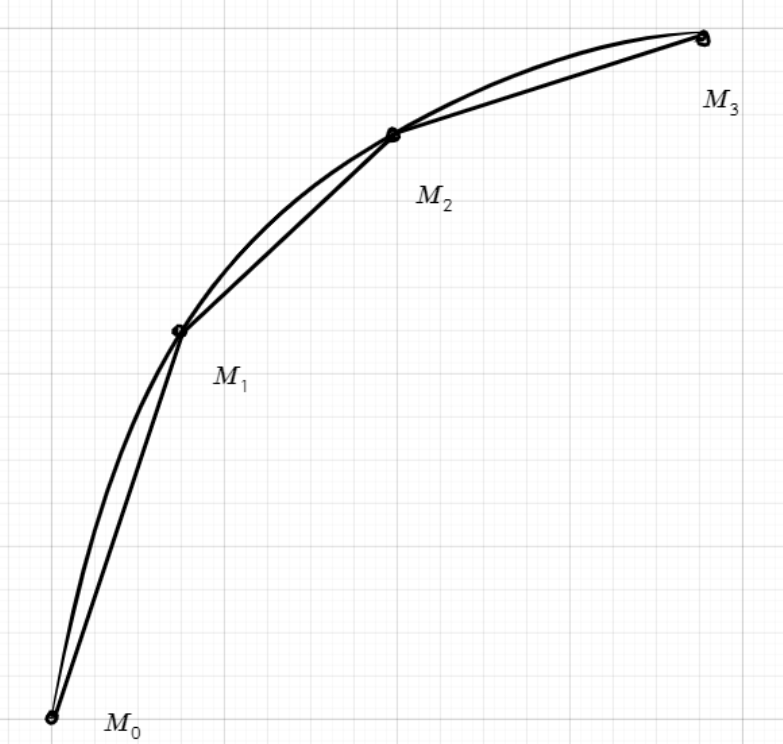
\includegraphics[scale=0.4]{images/img44.png}$$
Рассмотрим точки кривой $M_k$ = $M(x(t_k),y(t_k))$. Можно сказать, что разбиению \{$t_k$\} отрезка $[\upalpha;\upbeta]$ отвечает разбиение кривой $l$ точками $M_k$. Соединим последовательно точки $M_k$ между собой. Получим ломаную $M_0M_1M_2\dotso M_{n-1}M_n$.  Эта ломаная вписана в кривую $l$. Длина ломаной равна сумме длин составляющих её отрезков:\\
$${L}_n = \sum\limits_{k=1}^n M_{k-1}M_k.$$
$\bullet$ \textit{Если множество длин ломаных, отвечающих всевозможным разбиениям отрезка} $[\upalpha;\upbeta]$,\textit{ а, следовательно, и всевозможным вписанным ломаным, ограничено сверху, то кривую $l$ называют \textbf{спрямляемой}, а число $s::=\sup\{{L}_n\}$ называют \textbf{длиной кривой $l$}}.
\begin{theorem}
	Гладкая кривая $l$: $\begin{cases}
		x=x(t),\\    
		y=y(t)
	\end{cases}$,  $t\in[\upalpha;\upbeta]$ спрямляема и её длина может быть вычислена по формуле
	$$s = \int\limits_\upalpha^\upbeta \sqrt{\dot x^2(t) + \dot y^2(t)}dt.$$
\end{theorem}
\begin{Proof}
	Длина $L_k$ звена ломаной $M_{k-1}M_k$ может быть вычислена следующим образом:\\\\
	$L_k = \sqrt{(x(t_k)-x(t_{k-1}))^2 + (y(t_k)-y(t_{k-1}))^2}$ = [по формуле конечных приращений] = \\\\ = $\sqrt{(\dot x(\tau_k)\Delta t_k)^2 + (\dot y(\tilde \tau_k)\Delta t_k)^2}$ = $((\dot x(\tau_k))^2 + (\dot y(\tilde \tau_k))^2)^{\frac12} \Delta t_k$ = $(\dot x^2(\tau_k) + \dot y^2(\tau_k))^{\frac12} \Delta t_k + \\ \\
	+ \underbrace{((\dot x^2(\tau_k) + \dot y^2(\tilde \tau_k))^{\frac12} - (\dot x^2(\tau_k) + \dot y^2(\tau_k))^{\frac12}) \Delta t_k}_{A_k}$\\\\
	Теперь преобразуем ${A_k}$, домножив и разделив на сопряжённое:\\\\
	${A_k}$ = $\dfrac{\dot x^2(\tau_k) + \dot y^2(\tilde \tau_k) - \dot x^2(\tau_k) + \dot y^2(\tau_k)}
	{(\dot x^2(\tau_k) + \dot y^2(\tilde \tau_k))^{\frac12} + (\dot x^2(\tau_k) + \dot y^2(\tilde \tau_k))^{\frac12}} \Delta t_k$ = 
	$\dfrac{(\dot y(\tilde \tau_k) - \dot y(\tau_k)) (\dot y(\tilde \tau_k) + \dot y(\tau_k) )}
	{(\dot x^2(\tau_k) + \dot y^2(\tilde \tau_k))^{\frac12} + (\dot x^2(\tau_k) + \dot y^2(\tilde \tau_k))^{\frac12}} \Delta t_k$\\\\
	Оценим ${A_k}$:\\\\
	${|A_k|}$ 
	$\leqslant$
	$|\dot y(\tilde \tau_k) - \dot y(\tau_k)| \cdot
	\underbrace{\frac{|\dot y(\tilde \tau_k) + \dot y(\tau_k)|}
		{(\dot x^2(\tau_k) + \dot y^2(\tilde \tau_k))^{\frac12} + (\dot x^2(\tau_k) + \dot y^2(\tilde \tau_k))^{\frac12}}}_{\leqslant 1} \Delta t_k$ 
	$\leqslant$ 
	$|\dot y(\tilde \tau_k) - \dot y(\tau_k)|\cdot \Delta t_k$\\\\
	Для всей длины ломаной будем иметь: 
	$${L} = \sum\limits_{k=1}^n M_{k-1}M_k = \sum\limits_{k=1}^n (\dot x^2(\tau_k) + \dot y^2(\tau_k))^{\frac12}\Delta t_k + \sum\limits_{k=1}^n A_k \eqno(1)$$\\
	Оценим $\left|\sum\limits_{k=1}^n A_k\right| \leqslant \sum\limits_{k=1}^n |A_k| 
	\leqslant 
	\sum\limits_{k=1}^n
	|\dot y(\tilde \tau_k) - \dot y(\tau_k)|\cdot \Delta t_k$\\\\
	По условию $\dot y(t)$ непрерывна на отрезке $ [\upalpha;\upbeta] $.
	На основании теоремы Кантора она и равномерно непрерывна. Следовательно, при достаточно мелком разбиении отрезка $ [\upalpha;\upbeta] $ при $\forall \varepsilon > 0$ будет выполняться $|\dot y(\tilde \tau_k) - \dot y(\tau_k)| \leqslant \varepsilon$.\\\\ Подробнее: $\forall \varepsilon > 0$, $\exists \delta (\varepsilon) > 0$. Такое что $ \forall \{t_k\} $ с диаметром $\delta \leqslant \delta_{\varepsilon} $  $\Rightarrow$  $|\dot y(\tilde \tau_k) - \dot y(\tau_k)| \leqslant \varepsilon$, $\forall k$.\\ Поэтому $\left|\sum\limits_{k=1}^n A_k\right| \leqslant \sum\limits_{k=1}^n \varepsilon \cdot \Delta t_k = \varepsilon (b-a) \Rightarrow \sum\limits_{k=1}^n A_k \longrightarrow 0$ при $\delta \longrightarrow 0$.\\\\
	Следовательно ${L} \underset{\delta \rightarrow 0} \longrightarrow \int\limits_\upalpha^\upbeta \sqrt{\dot x^2(t) + \dot y^2(t)}dt$. \\
	Поэтому $s=\sup\{{L}\} \geqslant \int\limits_\upalpha^\upbeta \sqrt{\dot x^2(t) + \dot y^2(t)}dt$.\\\\
	С другой стороны, какую бы фиксированную ломаную мы ни взяли, её длина от добавления новых точек деления только увеличивается. Поэтому ${L} \leqslant \lim\limits_{\delta \to 0}{L} = \int\limits_\upalpha^\upbeta \sqrt{\dot x^2(t) + \dot y^2(t)}dt $ и $s=\sup\{{L}\} \leqslant \int\limits_\upalpha^\upbeta \sqrt{\dot x^2(t) + \dot y^2(t)}dt$.\\
	Сопоставляя, заключаем, что $s = \int\limits_\upalpha^\upbeta \sqrt{\dot x^2 + \dot y^2}dt$. 
\end{Proof}
\begin{corollary}
	\begin{enumerate}
		\item
		Если кривая $\Gamma_f$ задана явным уравнением $y=f(x)$, $x\in [\upalpha; \upbeta]$, то $\begin{cases}
			x=x , \\
			y=f(x)
		\end{cases}$, $x\in [a; b]$ --- её параметрические уравнения и, применяя теорему имеем:
		$$s = \int\limits_a^b \sqrt{1 + f'^2(x)}dx.$$
		\item
		Если кривая задана полярным уравнением $r=r(\varphi)$, $\varphi \in [\upalpha;\upbeta]$, что нетрудно написать её параметрические уравнения:\\
		$\begin{cases}
			x= r(\varphi) \cos\varphi, \\
			y= r(\varphi) \sin\varphi
		\end{cases}$ $\varphi \in [\upalpha;\upbeta]$\\\\
		Тогда $\dot x^2 + \dot y^2 = (r'(\varphi)\cos\varphi - r(\varphi)\sin\varphi)^2 + (r'(\varphi)\sin\varphi + r(\varphi)\cos\varphi)^2 = r^2(\varphi) + r'^2(\varphi)$  и, поэтому
		$$s = \int\limits_\upalpha^\upbeta \sqrt{r^2(\varphi) + r'^2(\varphi)}d\varphi.$$
		\item
		Для пространственной кривой формула может быть получена по аналогии с плоской и имеет следующий вид:
		$$s = \int\limits_\upalpha^\upbeta \sqrt{\dot x^2 + \dot y^2 + \dot z^2}dt.$$
	\end{enumerate}
\end{corollary}
\section{Дифференциал дуги.}
Обозначим $s(t)$ длину дуги кривой от точки $M(\upalpha)$ до точки $M(t)$.
Тогда $$s(t) = \int\limits_\upalpha^t\sqrt{\dot x^2(\tau)+ \dot y^2(\tau)}d\tau .$$
По теореме Барроу:\\\\
$$s'(t) = \sqrt{\dot x^2(t)+ \dot y^2(t)}.$$
Следовательно $ds(t) = s'(t)dt = \sqrt{\dot x^2(t)+ \dot y^2(t)}dt = \sqrt{dx^2 + dy^2}$.
$$ds = \sqrt{dx^2 + dy^2}.$$
Изучим, что означает это равенство геометрически. $ds$ --- длина хорды, стягивающей две точки кривой.
$$\Delta s = ds + o(\Delta t).$$
\textit{Таким образом, бесконечно малая дуга по длине эквивалентна хорде, стягивающей её концы.}
\section{Квадрируемые фигуры}
$\bullet$ \textit{\textbf{Плоская фигура} --- это произвольное множество точек плоскости.}\\\\
$\bullet$ \textit{\textbf{Граничной точкой} $M$ фигуры $\underline{P}$ называют точку, в любой окрестности которой, то есть в любом круге положительного радиуса с центром в точке $M$ лежат как точки фигуры $P$, отличные от $M$, так и точки, не принадлежащие фигуре.}\\\\
$\bullet$ \textit{Совокупность всех граничных точек называют \textbf{границей фигуры} $P$.
	Обозначать границу будем символом $\partial \underline{P}$}\\\\
Рассмотрим треугольник $T$ с вершинами $M_k(x_k; y_k)$, $k = 1, 2, 3$.\\
Число $S_\text{тр}::=\frac12 \left|\begin{vmatrix}
	x_1& y_1 & 1\\
	x_2& y_2 & 1 \\
	x_3& y_3 & 1
\end{vmatrix}\right| = \frac12 \left|\begin{vmatrix}
	x_1 - x_3 & y_1 - y_3 \\
	x_2 - x_3 & y_2 - y_3
\end{vmatrix}\right|$ \\даёт площадь треугольника и его можно аксиоматически взять за определение площади.\\\\
$\bullet$ \textit{\textbf{Многоугольником} будем называть фигуру, которую можно представить как объединение конечного числа треугольников, которые могут иметь общими только граничные точки.}\\\\
$\bullet$ \textit{\textbf{Площадью многоугольника} назовём сумму площадей составляющих его треугольников.}\\\\
Из свойств определителей следует, что величина площади многоугольника не зависит от способа разбиения оного на треугольники.\\\\
Рассмотрим теперь произвольную фигуру $\underline{P}$, предполагая её ограниченной, то есть такой, что $\sup M_1 M_2 $ \textless $ +\infty$, $\forall M_1 M_2 \in \underline{P}$ (она расположена внутри некоторого многоугольника)\\\\
$\bullet$ \textit{Многоугольник $D^*$ будем называть \textbf{описанным} около фигуры $P$, если $P\subset D^*$.}\\\\
$\bullet$ \textit{Многоугольник $D_*$ будем называть \textbf{вписанным} в фигуру $P$, если $D_* \subset P$.}
$$D_* \subset P \subset D^*.$$
$$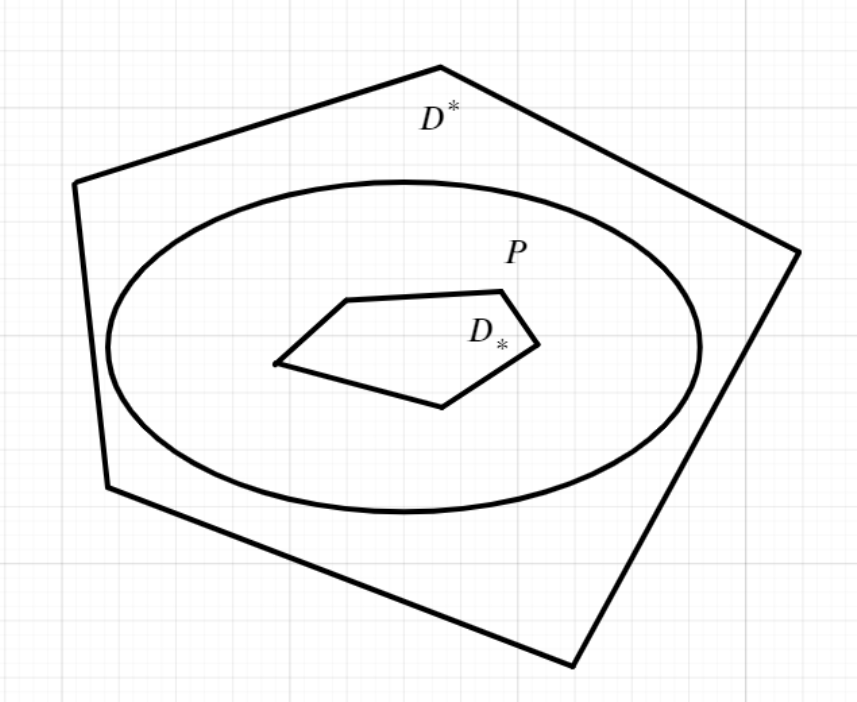
\includegraphics[scale=0.5]{images/img45.png}$$
Площадь $D^* \geqslant 0$ (множество ограничено снизу) $\Rightarrow$ $\exists S^*::=\inf\{\text{пл.}$ $D^*\} \geqslant 0 $\\
Вся $D_*$ лежит внутри каждого из $D^*$, поэтому $\{\text{пл.}$ $D_*\}$ ограничено сверху.
Обозначим $S_*::=\sup\{\text{пл.}$ $D_*\}.$
По построению $S^* \leqslant S_*$\\\\
$\bullet$ \textit{Если $S^* = S_*$, то фигуру $P$ называют \textbf{квадрируемой}, а число $S = S_* = S^*$ называют её \textbf{площадью}.}\\\\
Приведём несколько очевидных утверждений:
\begin{enumerate}
	\item \textit{Если имеется последовательность вписанных многоугольников и последовательность описанных многоугольников, последовательности площадей которых имеют общий предел $\mathcal{S}$, что фигура $\underline{P}$ квадрируема и её площадь равна $\mathcal{S}$.}
	\item \textit{Если $\forall \varepsilon > 0$, $\exists D^*$, $D_*$ такие, что $\text{пл.}D^* - \text{пл.}D_* \leqslant \varepsilon $, то $\underline{P}$ квадрируема.}
	\item \textit{Если $\forall \varepsilon > 0$, $\exists$ квадрируемые фигуры $P_*$, $P^*$ такие, что $P_* \subset P \subset P^*$ и $\text{пл.}P^* \text{ --- пл.}P_* \leqslant \varepsilon $ $\Rightarrow$ $P$ --- квадрируема.}
	\item \textit{Для квадрируемости $P$ $\Longleftrightarrow$ чтобы площадь границы $\partial P$ этой фигуры была равна нулю.\\
	Это следует из того, что, исключив из $D^*$ точки $D_*$ получим многоугольник, содержащий границу $\partial \underline{P}$.}
	\item \textit{При вращении, параллельном переносе, а также при преобразовании симметрии площади фигур не меняются.}
\end{enumerate}
Площадь является аддитивной характеристикой фигуры. Если взять разбиение фигуры на квадрируемые части, то площадь всей фигуры равна сумме площадей составляющих её частей.\\\\
Длина $-$ также аддитивная характеристика кривой.\\\\
Пример неквадрируемой фигуры. Выбросим все точки с рациональными абсциссами.
$$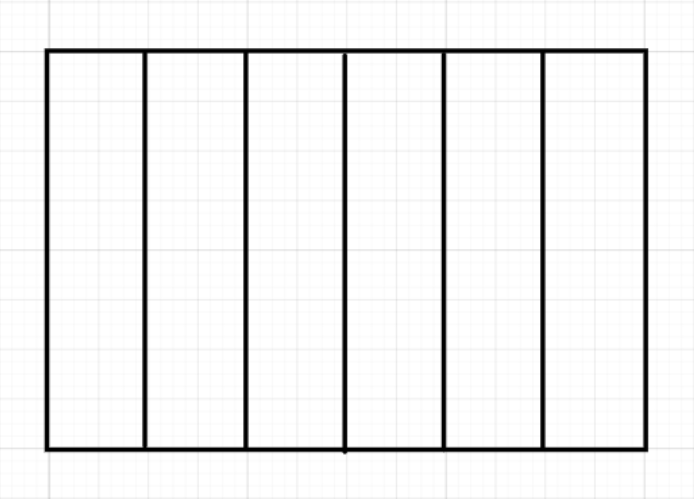
\includegraphics[scale=0.5]{images/img46.png}$$
\section{Кубируемые тела.}
$\bullet$ \textit{\textbf{Тело} --- пространственная фигура --- любое $\forall$ множество точек в $\mathbb{R}^3$.}\\\\
Теория строится по аналогии с плоским случаем.\\\\
Возьмём четыре точки $M_k(x_k, y_k, z_k)$, $k=1, 2, 3, 4$ и построим тетраэдр $T$ с вершинами в этих точках (симплекс)
$$ T = \{ M | M = \sum\limits_{k=1}^n \tau_k M_k, \forall \tau_k, \tau_k \geqslant 0, \sum\limits_{k=1}^n \tau_k = 1\}$$
$\bullet$ \textit{\textbf{Объёмом тетраэдра} назовём число 
	$\text{об.}T = \frac{1}{3!}\left| \begin{vmatrix}
		x_1& y_1 & z_1 & 1\\
		x_2& y_2 & z_2 & 1 \\
		x_3& y_3 & z_3 & 1  \\
		x_4& y_4 & z_4 & 1 
	\end{vmatrix}\right| $}\\\\
$\bullet$ \textit{\textbf{Многогранник} $-$ тело, представляющее собой объединение конечного числа тетраэдров, имеющих общими только точки границы.}\\\\
$\bullet$ \textit{\textbf{Объём многогранника} $-$ сумма объёмов составляющих его тетраэдров.}\\\\
Рассмотрим тело $\underline{P}$ и многогранники описанные $D^*$ и вписанные $D_*$ в это тело.\\
$V^* = \inf\{\text{об.}D^*\}$  ;  $V_* = \sup\{\text{об.}D_*\}$\\\\
$\bullet$ \textit{Если $V_* = V^*$, то тело $P$ называют \textbf{кубируемым}, а $V = V_* = V^*$ --- его \textbf{объёмом}.}\\\\
\textit{Для кубируемости тела $\Longleftrightarrow$ чтобы его граница имела нулевой объём, то есть $\forall \varepsilon > 0$ эту границу можно было заключить в многогранник, объём которого $\leqslant \varepsilon$.}\\
и т. д.
\chapter{Некоторые приложения интеграла.}
\section{Геометрический смысл определенного интеграла.}
$$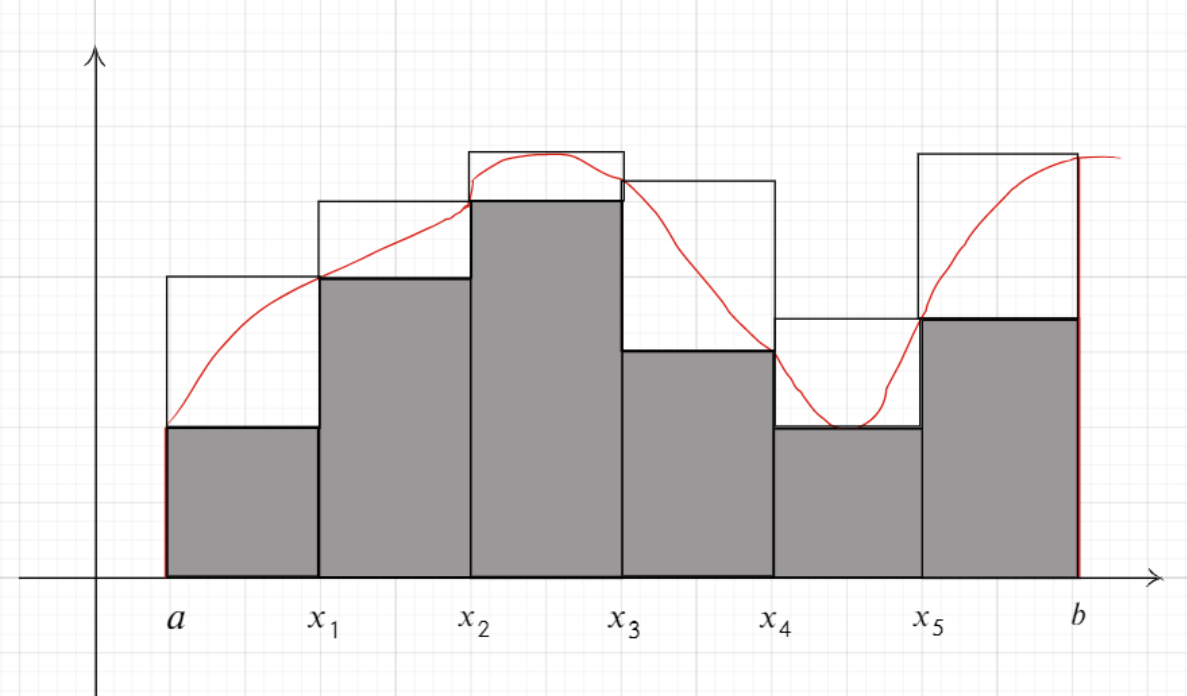
\includegraphics[scale=0.5]{images/img47.png}$$
Пусть $f:[a;b]\ra\Rm$, непрерывна и неотрицательна на $[a;b]$.\\\\
$\bullet$ \textit{Фигуру $P = \{(x;y) | a\leq x\leq b; 0\leq y\leq f(x)\}$ будём называть \textbf{криволинейной трапецией}.}\\\\
Возьмём разбиение $\{x_k\}$ отрезка $[a;b]$ с диаметром $\delta$. На основании теоремы Вейерштрасса всегда можно выбрать точку максимума $\overline{\theta_k} \in [x_{k-1}; x_k]$ и точку минимума $\underline{\theta_k}\in[x_{k-1};x_k]$ функции $f$ на отрезке $[x_{k-1}; x_k].$\\\\
Интегральные суммы:
$$\overline{\sigma} = \sum_{k=1}^{n}f(\overline{\theta_k})\Delta x_k\quad\text{и}\quad \underline{\sigma}=\sum_{k=1}^{n}f(\underline{\theta_k})\Delta x_k$$
дают площади многоугольников, составленных из прямоугольников. Первый из этих многоугольников описан около криволинейной трапеции, а второй --- вписан в неё.\\\\
Нa основании теоремы об интегрируемости непрерывной функции величины $\overline{\sigma}$ и $\underline{\sigma}$ при $\delta\ra0$ имеют общий предел $s = \int_a^b f(x)dx$, который является площадью криволинейной трапеции.\\\\
Полученный результат обобщается и на другие ситуации.
Например, если $f<0$, то $s = -\int_a^b f(x)dx$.
В общем случае s = $\int_a^b|f(x)|dx$.
Если $s = \int_a^b|f(x)-g(x)|dx$
\section{Площадь криволинейного сектора}
$r = r(\varphi), \varphi\in[\alpha;\beta]$\\
Разбиваем $[\alpha;\beta]$ на $n$ частей точками $\varphi_k$.\\
$\underline{\varphi_k}$ - точка минимума $r(\varphi)$\\
$\overline{\varphi_k}$ - точка максимума $r(\varphi$\\
Круговой сектор квадрируем.\\
Описанный круговой сектор для выделенной фигуры имеет площадь $\frac{1}{2} r^2(\overline{\varphi_k})\Delta\varphi_k$,\\
вписанный --- площадь $\frac{1}{2} r^2(\underline{\varphi_k})\Delta\varphi_k$.\\
Фигура, составленная из конечного числа круговых секторов --- квадрируема.